\documentclass[11pt]{exam}
\usepackage{amsmath,amssymb}
\usepackage[empty]{fullpage}
\usepackage{tikz}
\usetikzlibrary{decorations.pathmorphing,patterns}
\usepackage{soul}

\newcommand{\ds}{\displaystyle}

\begin{document}
\subsection*{Project 3 \hfill Math 243}

\noindent
\textit{Type your solutions using Microsoft Word, Google Docs, or LaTeX (or other document editor). Either print your solutions or send me a PDF file by class on \textbf{Friday, Dec 5}. Your grade will be based on three factors: completeness, correctness, and style. To get full style credit you should write all answers in complete sentences. You may work with a partner and submit one project together, if you prefer. It is okay to discuss the problems with other students, but all of your solutions must be explained in your own words. }  \\

%Suppose a small satellite orbits a large planet.  The mass of the planet is so much larger than the satellite that we can assume that the planet is stationary at the origin $(x,y,z) = (0,0,0)$, and only the satellite is moving.  Although the satellite can move in three dimensions $x$, $y$, and $z$, we'll assume that the z-component of the satellite is always zero, so all of the satellite's motion takes place on the $(x,y)$-plane. 

A \textbf{tuned mass damper} (TMD) is a device that consists of a mass mounted on damped springs that are attached to a larger structure in order to reduce mechanical vibrations. TMDs are used in cars, buildings, bridges, and even medical equipment.  The idea is that if the oscillation frequency of the TMD is tuned to be similar to the resonance frequency of the structure it is attached to, then this will reduce the maximum amplitude of oscillations in the structure.  

A simplified example of a TMD can be seen in the figure below.  A large mass $m_1$ is attached to a wall by a damped spring.  A second damped spring attaches a smaller mass $m_2$ to the first mass. The second spring and mass represent the tuned mass damper.  Outside forces represented by $f(t)$ push against the first mass.  By choosing the right spring constant $k_2$ and damping coefficient $c_2$ for the second spring, hopefully we'll be able to control the amplitudes of the oscillation of the mass $m_1$. 

\begin{center}
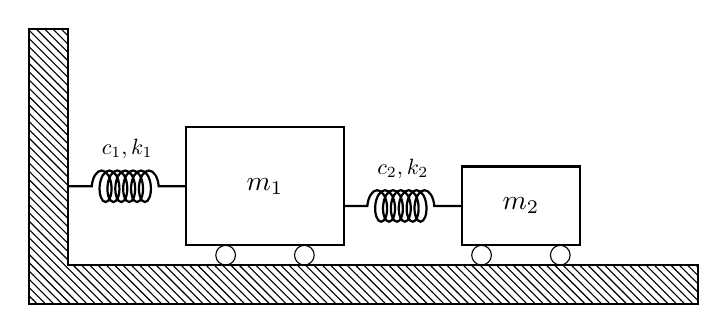
\begin{tikzpicture}
\filldraw[fill=gray!30,pattern=north west lines, thick] (-0.5,-0.5) -- (-0.5,3) -- (0,3) -- (0,0) -- (8,0) -- (8,-0.5) -- cycle;
\draw[thick] (1.5,0.25) rectangle (3.5,1.75);
\draw[thick] (5.0,0.25) rectangle (6.5,1.25);
\draw (2,0.125) circle (0.125);
\draw (3,0.125) circle (0.125);
\draw (5.25,0.125) circle (0.125);
\draw (6.25,0.125) circle (0.125);
\draw[decoration={
		coil,
		segment length = 1mm,
		amplitude = 2mm,
		aspect = 0.5,
		post length = 3mm,
		pre length = 3mm},
	decorate, thick] (0,1) -- (1.5,1);
\draw[decoration={
		coil,
		segment length = 1mm,
		amplitude = 2mm,
		aspect = 0.5,
		post length = 3mm,
		pre length = 3mm},
	decorate, thick] (3.5,0.75) -- (5,0.75);
\draw (2.5,1) node {$m_1$};
\draw (5.75,0.75) node {$m_2$};
\draw (0.75,1.25) node[above,scale=0.8] {$c_1, k_1$};
\draw (4.25,1.0) node[above,scale=0.8] {$c_2, k_2$};
\end{tikzpicture}

\end{center}

Using Newton's second law, the horizontal position $x_1$ of the first mass satisfies:
$$m_1 x_1'' = -k_1 x_1 + k_2(x_2 - x_1) - c_1 x_1' + c_2(x_2' - x_1') + f(t)$$
and the position $x_2$ of the second mass satisfies: 
$$m_2 x_2'' = -k_2(x_2 - x_1) - c_2 (x_2' - x_1')$$
where $x_1$ and $x_2$ measure how far each mass is away from its resting position.  You can assume that the masses are small enough and there is enough space between them for $x_1$ and $x_2$ to get large without them colliding (or hitting the wall). 

\begin{questions}
\question \textbf{Set up the system.} Convert the system of two second order equations above into a system of four first order equations involving the velocities $x_1'$ and $x_2'$ and the positions $x_1$ and $x_2$.  Then re-write the system in matrix form $\mathbf{y}' = A \mathbf{y} + \mathbf{f}(t)$ where $\mathbf{y} = \langle x_1, x_1', x_2, x_2' \rangle$.  What is the matrix $A$ and the vector-valued forcing function $\mathbf{f}(t)$? 

\begin{solution}
\begin{align*}
y_1' &= y_2 \\
y_2' &= -\tfrac{k_1}{m_1} y_1 + \tfrac{k_2}{m_1} (y_3 - y_1) - \tfrac{c_1}{m_1} y_2 + \tfrac{c_2}{m_1} (y_4 - y_2) + f(t) \\
y_3' &= y_4 \\
y_4' &= -\tfrac{k_2}{m_2}(y_3 - y_1) - \tfrac{c_2}{m_2} (y_4 - y_2)
\end{align*}
Translating this to a matrix equation, we have 
$$\mathbf{y}' = \begin{bmatrix} 
0 & 1 & 0 & 0 \\
-\tfrac{k_1}{m_1}  - \tfrac{k_2}{m_1} & \tfrac{c_1}{m_1} - \tfrac{c_2}{m_1} & \tfrac{k_2}{m_1} & \tfrac{c_2}{m_1} \\
0 & 0 & 0 & 1 \\ 
\tfrac{k_2}{m_2} & \tfrac{c_2}{m_2} & -\tfrac{k_2}{m_2} &- \tfrac{c_2}{m_2} 
\end{bmatrix} \mathbf{y} + \begin{bmatrix} 0 \\ f(t) \\ 0 \\ 0 \end{bmatrix}.$$

\end{solution}

\question \textbf{Find the undetermined coefficients.} Suppose that $m_1 = 100$, $m_2 = 1$, $c_1 = c_2 =0$, $k_1 = 900$ and $k_2 = 1$.  Suppose also that the forcing function is $f(t) = \cos 3t$ so that $\mathbf{f}(t) = \cos 3t \, \mathbf{e}_2$ where $\mathbf{e}_2 = \langle 0, 1, 0, 0 \rangle$.  To guess a particular solution for $\mathbf{y}' = A \mathbf{y} + \mathbf{f}(t)$, first switch to a complexified equation:
\[
\mathbf{y}' = A \mathbf{y} + e^{3i t} \mathbf{e}_2.
\]
Our guess is that the particular solution $\mathbf{y}_p$ will be the real part of $e^{3it} \, \mathbf{a}$ where $\mathbf{a}$ is a constant vector.  Show that if you substitute $e^{3it} \, \mathbf{a}$ into the complexified differential equation, then 
\[
\mathbf{a} = (3i I - A)^{-1} \mathbf{e}_2.
\]

\question \textbf{Find a particular solution.} Use a computer to find the real part of $e^{3it} \, \mathbf{a}$.

\question \textbf{Solve the IVP.} To solve a non-homogeneous linear system $\mathbf{y}' = A \mathbf{y} + \mathbf{f}(t)$ with initial conditions, you can use the matrix exponential.  The solution to the system is 
\begin{equation*}
\mathbf{y}(t) = e^{At} (\mathbf{y}(0) - \mathbf{y}_p(0)) + \mathbf{y}_p(t)
\end{equation*}
where $\mathbf{y}(0)$ is the initial condition and $\mathbf{y}_p(t)$ is any particular solution of the system. Suppose that our initial conditions are $\mathbf{y}(0) = \langle 0, 0, 0, 0 \rangle$. Find a formula for $\mathbf{y}(t)$. I recommend using Python with the \verb|sympy| library.

\question \textbf{Graphical analysis.} Graph the value of $x_1(t)$ (the first entry of $\mathbf{y}(t)$) as a function of time for $0 \le t \le 50$.  What phenomenon appears to be happening in the graph? Explain. 


%If the forcing function $\mathbf{f}(t) = \mathbf{v} \cos \omega t$, then you can complexify and guess that the particular solution will be the real part of something that has the form $\mathbf{y}_p(t) = \mathbf{a} e^{i \omega t}$ where $\mathbf{a}$ is a constant vector.  Show that if you substitute $\mathbf{a} e^{i \omega t}$ into the complexified differential equation $\mathbf{y}' = A \mathbf{y} + \mathbf{v} e^{i \omega t}$, then you get 
%$$\mathbf{a} = (i \omega I - A)^{-1} \mathbf{v}$$

%Substituting this into the complexified system, we get 
%$$i \omega \mathbf{a} e^{i \omega t} - e^{i \omega t} A \mathbf{a} = \mathbf{v} e^{i \omega t}.$$
%Canceling the exponentials, we get
%$$(i \omega I - A) \mathbf{a} = \mathbf{v}$$
%so 
%$$\mathbf{a} = (i \omega I - A)^{-1} \mathbf{v}$$
%and therefore the particular solution is the real part of 
%$$(i \omega I - A)^{-1} \mathbf{v} e^{i \omega t}.$$

\question \textbf{Analyze the undamped case.} Try different values of the spring constant $k_2$ and see which values appear to do the best job keeping the amplitude of $x_1(t)$ under control.  Describe your findings and back up your results with some graphs and explanation.  Hint: the natural frequency of the first spring-mass pair is $\sqrt{k_1/m_1}$ and the natural frequency for the second spring-mass pair is $\sqrt{k_2/m_2}$.  

\question \textbf{Analyze the damped case.} What happens if the damping coefficient $c_1 = 30$?  How does that change the behavior of the system?  Once again, use graphs to explain your answer.  
\end{questions}

\end{document}






